\documentclass{article}

% if you need to pass options to natbib, use, e.g.:
%     \PassOptionsToPackage{numbers, compress}{natbib}
% before loading neurips_2018

% ready for submission
% \usepackage{neurips_2018}

% to compile a preprint version, e.g., for submission to arXiv, add add the
% [preprint] option:
%     \usepackage[preprint]{neurips_2018}

% to compile a camera-ready version, add the [final] option, e.g.:
     \usepackage[final]{neurips_2019}

% to avoid loading the natbib package, add option nonatbib:
%     \usepackage[nonatbib]{neurips_2018}

\usepackage[utf8]{inputenc} % allow utf-8 input
\usepackage[T1]{fontenc}    % use 8-bit T1 fonts
\usepackage{hyperref}       % hyperlinks
\usepackage{url}            % simple URL typesetting
\usepackage{graphicx}
\usepackage{booktabs}       % professional-quality tables
\usepackage{amsfonts}       % blackboard math symbols
\usepackage{nicefrac}       % compact symbols for 1/2, etc.
\usepackage{microtype}      % microtypography
\usepackage{listings}
\title{Applied Interpretable Inference: Connecting Probabilistic Programming with Epidemiology Simulators}

% The \author macro works with any number of authors. There are two commands
% used to separate the names and addresses of multiple authors: \And and \AND.
%
% Using \And between authors leaves it to LaTeX to determine where to break the
% lines. Using \AND forces a line break at that point. So, if LaTeX puts 3 of 4
% authors names on the first line, and the last on the second line, try using
% \AND instead of \And before the third author name.

\author{%
Paper ID: }
  % examples of more authors
  % \And
  % Coauthor \\
  % Affiliation \\
  % Address \\
  % \texttt{email} \\
  % \AND
  % Coauthor \\
  % Affiliation \\
  % Address \\
  % \texttt{email} \\
  % \And
  % Coauthor \\
  % Affiliation \\
  % Address \\
  % \texttt{email} \\
  % \And
  % Coauthor \\
  % Affiliation \\
  % Address \\
  % \texttt{email} \\
%}
\begin{document}
% \nipsfinalcopy is no longer used

\maketitle

\begin{abstract}

A goal of probabilistic programming is to couple simulators, with inference. This is 
because stochastic simulators are used prominently in many industrial settings,
do not require one to construct hand-crafted joint distributions as they implicitly 
define a joint distribution of the program and encode learnt structures 
directly. This makes simulators powerful tools and much of machine learning (ML) and 
Artificial Intelligence (AI)
can be seen as trying to emulate such simulators from a purely data-driven approach.
However, in the 
ML/AI setting, although we can often infer outcomes, we have little understanding about what 
in the data led to the outputted inferences. 
This makes it challenging to deploy ML/AI systems into the wild, especially in health-related and safety-critical domains, such
as epidemiology, as we lose \emph{interpretability}. 
In this work, we explain how to design ML/AI systems that combine
probabilistic programming systems (PPSs) and epidemiology simulators, to extract
fully interpretable posterior structures, enabling policy makers 
and practitioners to make interpretable inferences. 
In particular, we demonstrate this for the Malaria disease and show how we can 
perform interpretable inference in such settings.
\end{abstract}

\section{Introduction}

To do. 

\begin{itemize}

\item Outline the objectives
\item State the importance of interpretability in the inference of the simulator
\item Our system enables one to understand and interpret the most common paths in a program (simulation).
\item In highlighting this a practitioner can then go back to the field and explore that parameter/s in more depth.
\item This facilitates understanding and the construction of more detailed models and data collection strategies


\end{itemize}

% taken from Toms thesis. 

Stochastic simulators are common across a number of domains, statistical physics~\cite{landau_binder_2014}, financial modeling~\cite{jackel2002monte},
weather prediction~\cite{evensen1994sequential}, epidemiology~\cite{smith2008towards} and many others. 
An advantage of using stochastic simulators is that they provide a level of interpretability not found in modern deep learning settings, as they directly incorporate model structure from carefully reasoned observations and experiments.  
Probabilistic programming systems~(PPSs) are purpose built systems for making inferences and probabilistic 
modeling accessible. 
In particular, PPSs allow probabilistic models to be represented in the form of a generative model through the
probabilistic programming language~(PPL), which enables one to write statements that enable conditioning on data~\cite{gordon2014probabilistic,Goodman08church:a}. 
Thus, it seems only natural to connect simulators with PPSs, as simulators explicitly define a generative model, in the language in which they are written, and the nature of the PPSs enables us to perform inference in these simulators, by conditioning on observations, which are fed in as input to the simulators. 
In doing this we can infer things about stochastic input parameters and other variables sampled during the program's forward execution, whilst also providing full interpretability in the inference results, which is absolutely necessary in safety-critical domains.
By exploiting the tools that we develop in this paper, one is able to connect epidemiology simulators with \texttt{Pyprob}~\cite{le-2016-inference} to extract fully interpretable posterior structures allowing practitioners to interpret which input parameters have the largest affect on the epidemic, in our case malaria. Over five-hundred-thousand people die from malaria each year, mostly children under five years of age, with 90 per cent of malaria cases occurring in Sub-Saharan Africa. An estimated 100-300 million people suffer from malaria each year~\cite{world2016world}. 
Thus, by understanding the prominence of input parameters to epidemiology simulators, guides decision making processes relating to effective treatment and prevention strategies. 
\label{sec:related}


\section{Epidemiology Simulators and Probabilistic Programming}
\label{sec:background}
This will kind of be like a background section. 



\section{Methodology}
 TODO



Simulators encode several years, if not decades, of research and development and so by their very nature are structurally complicated. Since the development happens over several decades, usually without documentation, understanding a code base written with legacy libraries and software is incredibly difficult and an almost impossible task for a non-expert, or expert who has not had access to the previous years of development. Our method of hijacking simulators builds on the work of~\cite{baydin2018efficient} and extends the framework to encapsulate a more diverse range of simulators, in particular epidemiology simulators. Our framework provides a simple solution and makes it easy to transform arbitrary stochastic simulators into probabilistic programs, regardless of the complexity of the simulator and the language that the simulator is written in\footnote{The framework currently supports 9 popular languages, but there is nothing to stop this being extended to any language of interest.}. In addition to this, we can understand the structure of programs in simulators for both decoding \emph{black-box structures} and for posterior inference. This enables two things. 1) It enables software developers and researchers to understand complicated code bases. 2) It provides interpretable inference results that provide policy makers with predictions that are truly interpretable, in the sense that the end-user of the inference results understands what physical events led to inference outcome. This is critical in several domains, and is particularly important in the medical domain. 

\subsection{Connecting a Stochastic Simulator to a Probabilistic Programming System}

In order to hijack the stochastic simulator we are only required to override the location of the stochastic primitives, i.e. the operations that generate the stochasticity and randomness within the simulator. We will walk through how this is done for EMOD and OpenMalaria,  you will see that it is procedurally identical, however, given the sheer number of simulators it maybe slightly different procedurally. To our knowledge it shouldn't be, but we have not been able view of all simulators. 

\subsection{Extending Probabilistic Programming Protocols}

\begin{figure}[h!]
	\centering
	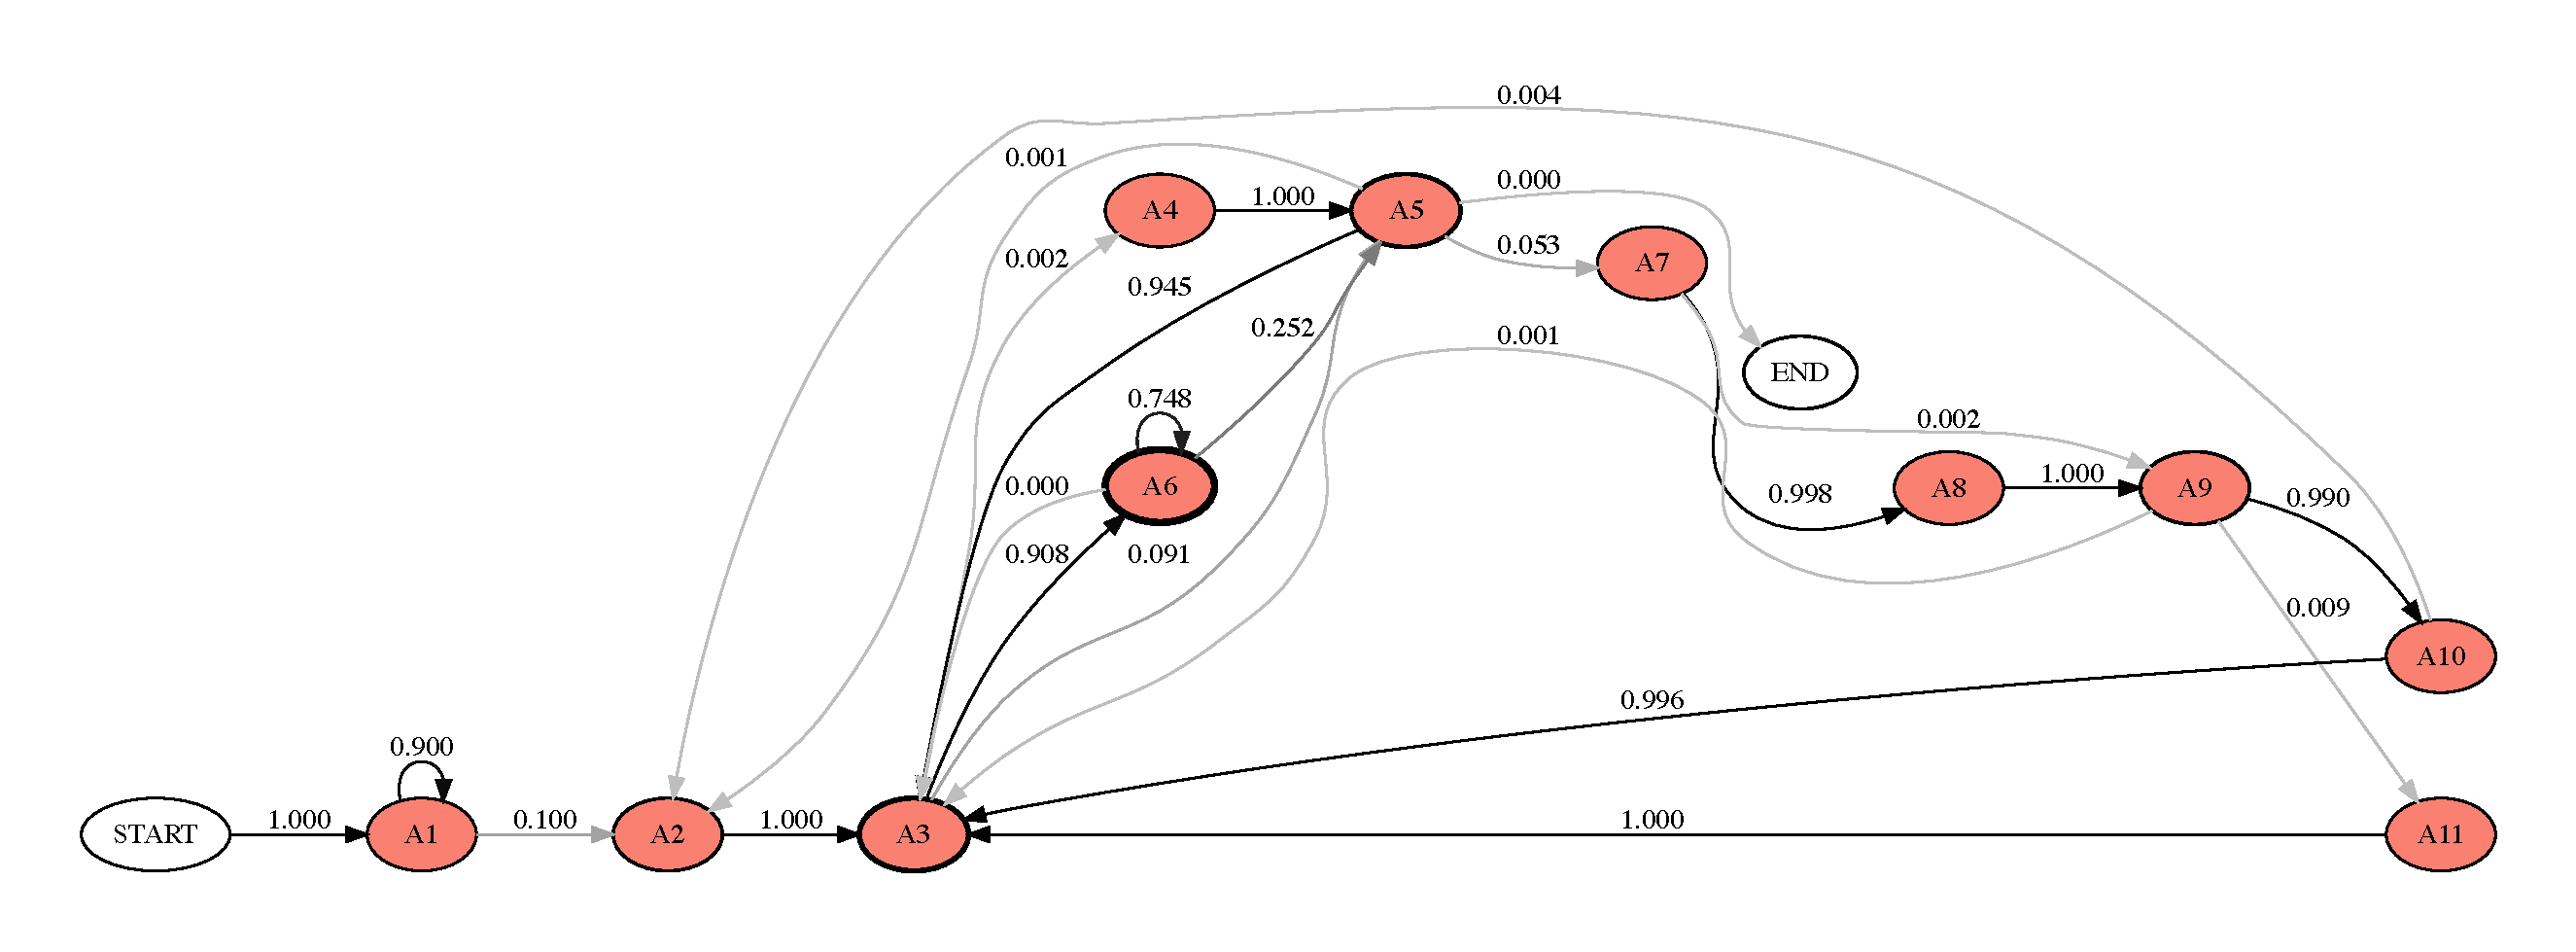
\includegraphics[width=\textwidth]{plots/ewan_25_pop_10.pdf}
	\caption{Add something. Population 10}
\end{figure}
\begin{figure}[h!]
	\centering
	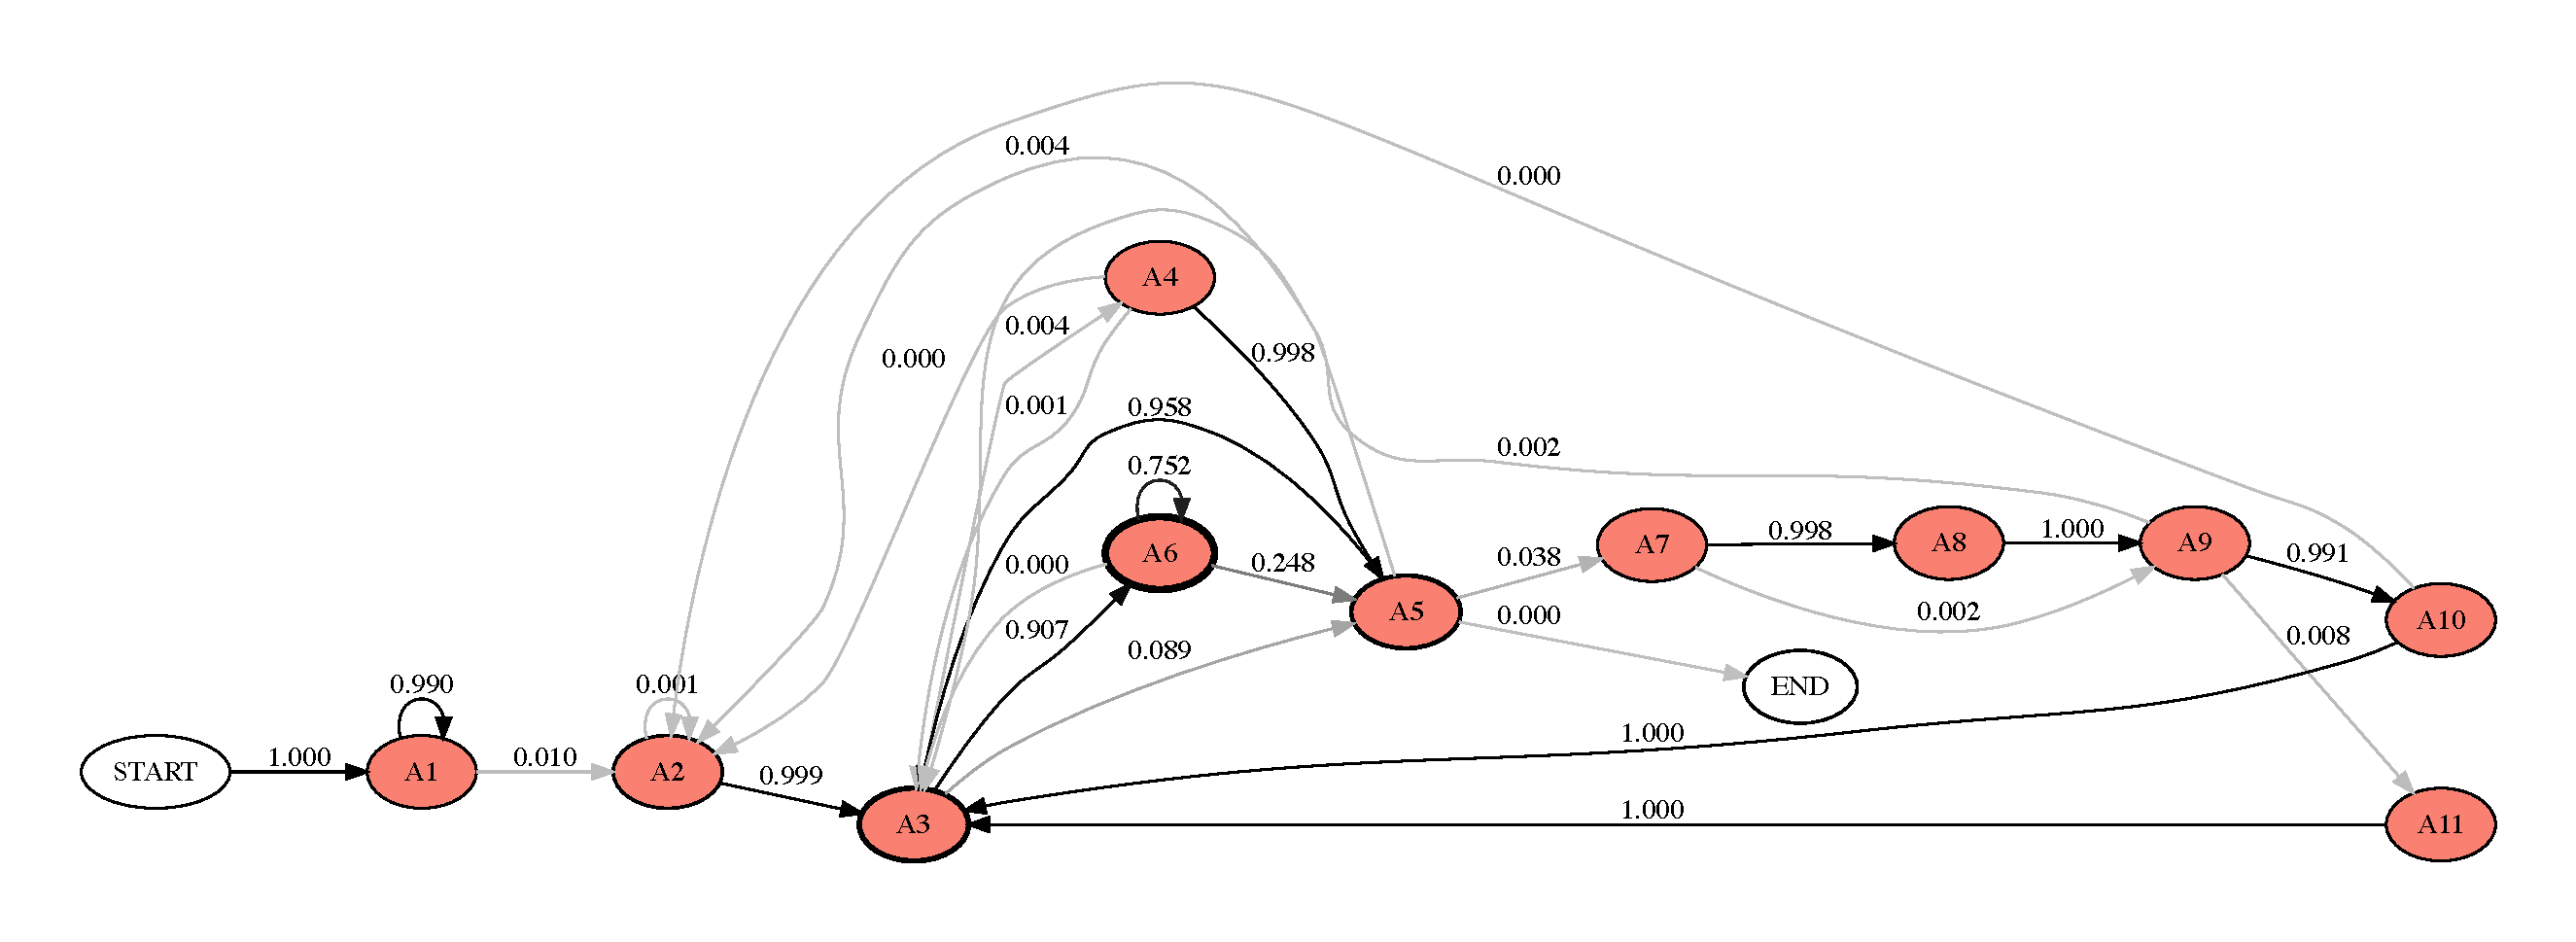
\includegraphics[width=\textwidth]{plots/ewan_25_pop_100.pdf}
	\caption{Add something. Population 100}
\end{figure}
TODO

\section{Results}

TO ADD


% \subsubsection*{Acknowledgments}

% Use unnumbered third level headings for the acknowledgments. All acknowledgments
% go at the end of the paper. Do not include acknowledgments in the anonymized
% submission, only in the final paper.

\section*{References}

\bibliographystyle{plain}
\bibliography{refs}

\end{document}